\documentclass[tikz,border=6pt]{standalone}
\usepackage{pgfplots}
\pgfplotsset{compat=1.18}
\usepgfplotslibrary{colormaps}
\usetikzlibrary{arrows, arrows.meta, calc}
\usetikzlibrary{decorations.markings}


\usepackage{amssymb,amsmath,mathtools}

\usepackage[T1]{fontenc}
\usepackage[utf8]{inputenc}
\usepackage{newpxtext,newpxmath}
\usepackage{sectsty}

\renewcommand{\Re}{\operatorname{\mathrm{Re}}}
\renewcommand{\Im}{\operatorname{\mathrm{Im}}}

\begin{document}
	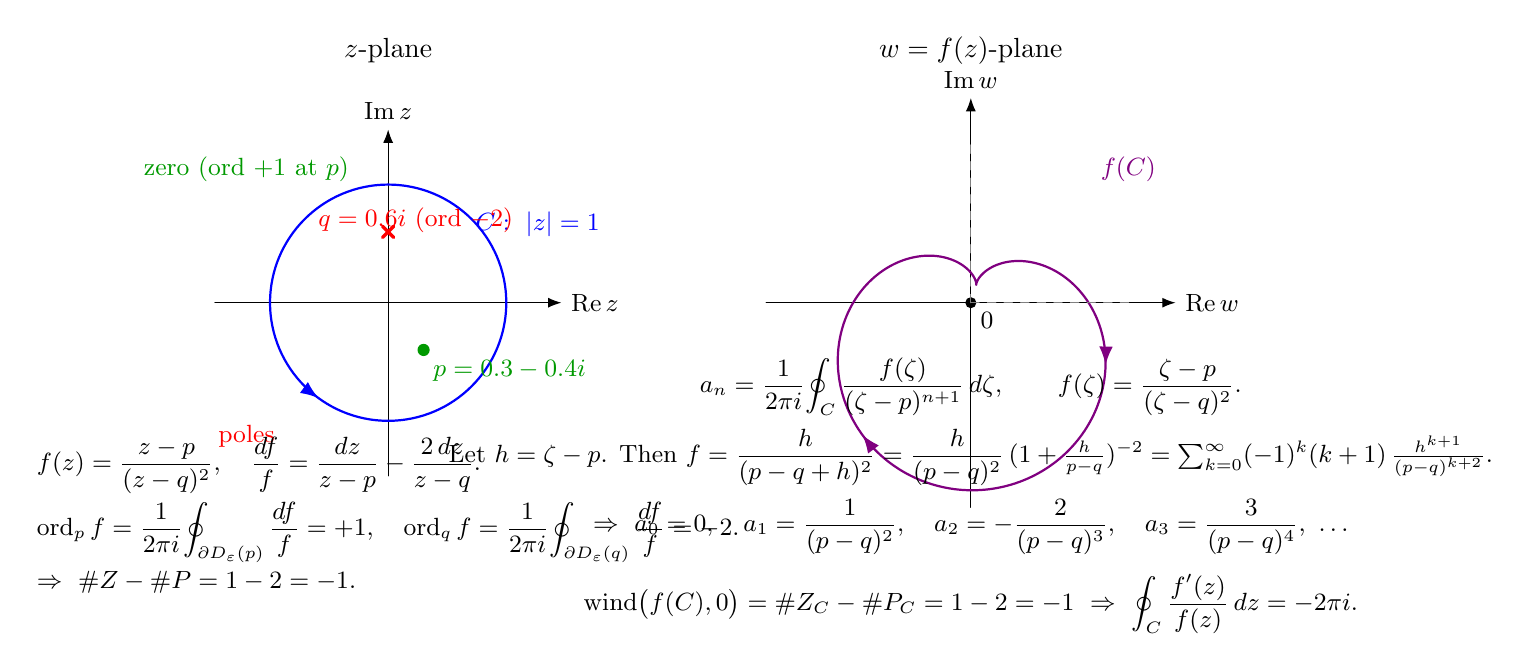
\begin{tikzpicture}[>=Latex, line cap=round, line join=round, font=\small]
		
		%========================
		% Left: z-plane
		%========================
		\begin{scope}[shift={(0,0)}]
			\node[font=\normalsize] at (0,3.2) {$z$-plane};
			% axes
			\draw[->] (-2.2,0)--(2.2,0) node[right] {$\Re z$};
			\draw[->] (0,-2.2)--(0,2.2) node[above] {$\Im z$};
			
			% unit circle C (positively oriented) -- radius 1.5 for visibility
			\draw[blue,thick,postaction={decorate},
			decoration={markings, mark=at position 0.65 with {\arrow{>}}}]
			(0,0) circle (1.5);
			\node[blue] at (1.9,1.0) {$C:\ |z|=1$};
			
			% zero at p (order +1) and pole at q (order -2)
			\fill[green!60!black] (0.45,-0.6) circle(2.2pt) node[below right] {$p=0.3-0.4i$};
			\node[green!60!black] at (-1.8,1.7) {zero (ord $+1$ at $p$)};
			\draw[red,very thick] (0,0.9) ++(-0.07,-0.07) -- ++(0.14,0.14);
			\draw[red,very thick] (0,0.9) ++(-0.07,0.07)  -- ++(0.14,-0.14);
			\node[red] at (0.35,1.05) {$q=0.6i$ (ord $-2$)};
			\node[red] at (-1.8,-1.7) {poles};
			
			% function label + orders via the winding / log-derivative form
			\node[align=left] at (0,-2.7) {$\displaystyle
				f(z)=\frac{z-p}{(z-q)^2},\quad
				\frac{df}{f}=\frac{dz}{z-p}-\frac{2\,dz}{z-q}.$\\[2pt]
				$\displaystyle \operatorname{ord}_{p} f=\frac{1}{2\pi i}\!\oint_{\partial D_\varepsilon(p)}\frac{df}{f}=+1,\quad
				\operatorname{ord}_{q} f=\frac{1}{2\pi i}\!\oint_{\partial D_\varepsilon(q)}\frac{df}{f}=-2.$\\[2pt]
				$\Rightarrow\ \#Z-\#P=1-2=-1.$};
		\end{scope}
		
		%========================
		% Right: w-plane = f(z)-plane
		%========================
		\begin{scope}[shift={(7.4,0)}]
			\node[font=\normalsize] at (0,3.2) {$w=f(z)$-plane};
			% axes
			\draw[->] (-2.6,0)--(2.6,0) node[right] {$\Re w$};
			\draw[->] (0,-2.6)--(0,2.6) node[above] {$\Im w$};
			
			% origin
			\fill (0,0) circle(2pt) node[below right] {$0$};
			
			% image curve f(C): z = 1.5 e^{it} -> w = (z-p)/(z-q)^2
			% Let x = 1.5 cos t, y = 1.5 sin t.
			% u = x - 0.3, v = y + 0.4  so  N = u + i v.
			% D = x + i(y - 0.6).  Then D^2 = A + i B with:
			%   A = x^2 - (y-0.6)^2,   B = 2 x (y-0.6).
			% So 1/D^2 = (A - iB)/(A^2+B^2), hence
			%   w = (u+iv)*(A - iB)/(A^2+B^2) has
			%   Re w = (uA + vB)/den,   Im w = (vA - uB)/den,   den = A^2 + B^2.
			\draw[violet,thick,
			postaction={decorate},
			decoration={markings,
				mark=at position 0.22 with {\arrow{>}},
				mark=at position 0.62 with {\arrow{>}}}]
			plot[domain=0:6.283, samples=720]
			({
				% Re w = (uA + vB)/den
				((1.5*cos(\x r)-0.3) *
				( (1.5*cos(\x r))*(1.5*cos(\x r)) - (1.5*sin(\x r)-0.6)*(1.5*sin(\x r)-0.6) )
				+ (1.5*sin(\x r)+0.4) *
				( 2*(1.5*cos(\x r))*(1.5*sin(\x r)-0.6) )
				)
				/
				(
				( (1.5*cos(\x r))*(1.5*cos(\x r)) - (1.5*sin(\x r)-0.6)*(1.5*sin(\x r)-0.6) )^2
				+ ( 2*(1.5*cos(\x r))*(1.5*sin(\x r)-0.6) )^2
				)
			},
			{
				% Im w = (vA - uB)/den
				((1.5*sin(\x r)+0.4) *
				( (1.5*cos(\x r))*(1.5*cos(\x r)) - (1.5*sin(\x r)-0.6)*(1.5*sin(\x r)-0.6) )
				- (1.5*cos(\x r)-0.3) *
				( 2*(1.5*cos(\x r))*(1.5*sin(\x r)-0.6) )
				)
				/
				(
				( (1.5*cos(\x r))*(1.5*cos(\x r)) - (1.5*sin(\x r)-0.6)*(1.5*sin(\x r)-0.6) )^2
				+ ( 2*(1.5*cos(\x r))*(1.5*sin(\x r)-0.6) )^2
				)
			});
			\node[violet] at (2.0,1.7) {$f(C)$};
			
			% dashed rays to visualize winding (here: -1, clockwise once)
			\draw[gray,dashed] (0,0) -- (2.1,0);
			\draw[gray,dashed] (0,0) -- (0,2.1);
			
			% annotation: Taylor coefficients at z_0=p via Cauchy integrals
			\node[align=center] at (0,-2.45)
			{$\displaystyle
				a_n=\frac{1}{2\pi i}\!\oint_C \frac{f(\zeta)}{(\zeta-p)^{n+1}}\,d\zeta,\qquad
				f(\zeta)=\frac{\zeta-p}{(\zeta-q)^2}.$\\[4pt]
				Let $h=\zeta-p$. Then $f=\dfrac{h}{(p-q+h)^2}
				=\dfrac{h}{(p-q)^2}\,(1+\tfrac{h}{p-q})^{-2}
				=\sum_{k=0}^{\infty}(-1)^k (k+1)\,\frac{h^{k+1}}{(p-q)^{k+2}}.$\\[4pt]
				$\Rightarrow\ a_0=0,\quad
				a_1=\dfrac{1}{(p-q)^2},\quad
				a_2=-\dfrac{2}{(p-q)^3},\quad
				a_3=\dfrac{3}{(p-q)^4},\ \ldots$\\[6pt]
				$\mathrm{wind}\big(f(C),0\big)=\#Z_C-\#P_C=1-2=-1
				\ \Rightarrow\
				\displaystyle \oint_C \frac{f'(z)}{f(z)}\,dz=-2\pi i.$};
		\end{scope}
		
	\end{tikzpicture}
\end{document}